% !TEX root = ../ClassicThesis_DEIB.tex

\chapter{Grape hardware and software Architecure} \label{chap:grapeSoftwareArchitecture}

In this chapter we are going to describe in a detailed way the architecture of the robotic platform we used to implement the system to fulfill the requirements described in Section \ref{sec:grapeProjectDescription}. First, in Section \ref{sec:grapeHwArch}, we are giving an overview of the hardware components, from the robot base to all the actuators/sensors present on board. In Section \ref{sec:grapeSwArch}, we'll start to analyze the software architecure of the system, explaining what the main modules are, and the relationships between them.

\section{GRAPE hardware architecture}\label{sec:grapeHwArch}

\subsection{Robotic Base}
The choice of the robotic base is, of course, a crucial point in the development of our system, for two reasons:
\begin{itemize}
	\item without a well-functioning robotic base, no other objective can be achieved
	\item the vineyard environment is particularly challenging in nature (this particular aspect will be well-justified in Chapter \ref{chap:localization}), so we cannot rely on a non-prudent choice.
\end{itemize}
As anticipated in Section \ref{sec:odometry}, the choice fell on the \textbf{Husky} \ac{UGV} from Clearpath Robotics\footnote{\url{https://www.clearpathrobotics.com/husky-unmanned-ground-vehicle-robot/}},
(see Figure \ref{fig:husky}). There are several reasons for the adoption of this specific model:
\begin{itemize}
	\item it's a widely used platform (\textit{e.g.}: \cite{husky1}; \cite{husky2}; \cite{husky3})
	\item it has a \textit{skid steering} kinematics that, as already seen in Section \ref{sec:odometry}, can be essentially reduced to a \textit{differential drive} kinematics, that is very simple.
	\item it's specifically designed for outdoor use, so robustness and ability to deal with unstructured terrain are problems addressed by its rugged construction and high-torque drivetrain.
	\item it offers a large payload capacity, to host the moltitude of sensors, actuators and computational units we need
	\item it's fully supported in \ac{ROS}, with open source drivers, configuration files and examples
\end{itemize}

\begin{figure}
	\centering
	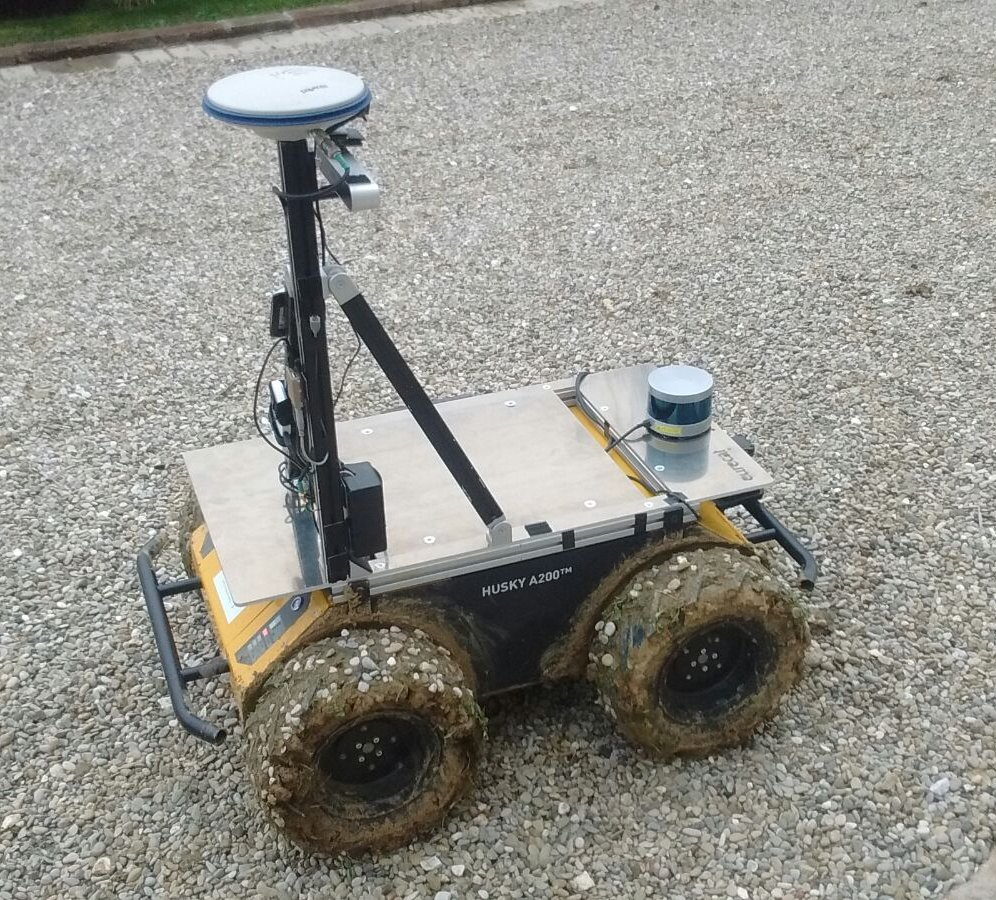
\includegraphics[width=0.5\textwidth]{Images/grape_sw_hw_architecture/ruoteFangose.jpeg}
	\caption{\textit{Husky platform after a navigation session in environment. You can easily note the amount of stones and mud stuck into the wheels.}}
	\label{fig:ruoteFangose}
\end{figure}

This choice turned out to be substantially good. The wheels odometry turned out to be  better than expected (TODO grafico della posizione xy dell'odometry delle ruote vs grafico della posizione stimata con robot localization), and the \ac{ROS} drivers and config files were actually pretty easy to use and modify. The only major weakness identified in the Husky is related to its behavior on muddy ground, and is due to the wheels shape. In effect, after a few minutes of navigation in the mud, the \ac{UGV} tends to collect a significative amount of earth and stones in the wheels groves (see Figure \ref{fig:ruoteFangose}) and, consequentely, lose grip on the ground. This problem is likely to be attenuated or solved by use of tracks instead of wheels.

\subsection{Robotic Arm}
By observing how pherormone dispensers must be deployed on the vine plant in Figure \ref{fig:dispensers} (in Figure \ref{fig:dispenserNostro}, you can see the dispenser shape that we actually used for \ac{GRAPE} project), it's easy to understand that we require a very flexible robotic arm, with advanced capacity of movement and capable of precise movement. Additional constraints also come from the limited space available on the Husky base, and from the limited power supply at disposal aboard. The choice fell on \textit{Jaco$^2$} arm from Kinova Robotics\footnote{\url{http://www.kinovarobotics.com/wp-content/uploads/2017/06/JACO\%C2\%B2-User-Guide-Asstive-Robotics-April-2017.pdf}}
(see Figure \ref{fig:kinovaArm}).

\begin{figure}
	\centering
	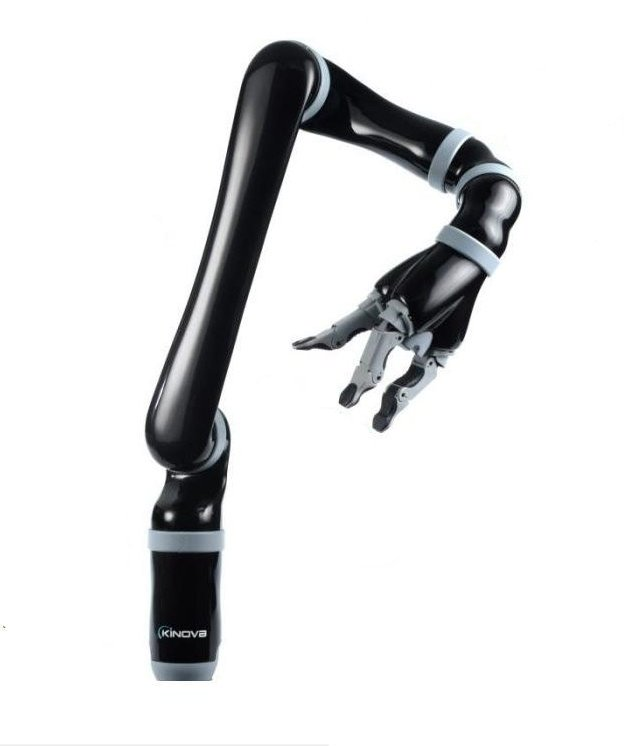
\includegraphics[width=0.6\textwidth]{Images/grape_sw_hw_architecture/kinova.jpg}
	\caption{\textit{Robotic arm Jaco$^2$ with 3 fingers, from Kinova Robotics.}}
	\label{fig:kinovaArm}
\end{figure}

COSA DEI DISABILI, UN PO' DI SPECIFICHE

\section{GRAPE sw architecture}\label{sec:grapeSwArch}


\begin{itemize}
\item Hardware del robot:
		\begin{itemize}
			\item scelta dell'husky (adatto per rugged terrain, supporto di pacchetti ROS), foto
			\item scelta del braccio, con pro (compatto, 6 dof, power consumption non elevata) e contro (movimenti non precisi, fragile, scarso controllo di collisione)
			\item lidar sul braccio per scan
			\item lidar davanti per navigazione e eventualmente localizzazione
			\item camera montata sul braccio
			\item velodyne davanti (a cosa serve?)
			\item camera fissa per eventualmente scattare foto alla vigna
			\item imu
		\end{itemize}
	\item foto del robot 
	%(http://www.grape-project.eu/wp-content/uploads/2017/11/20171030-MacchineTrattori.pdf e eventuali altre che faremo)

\item Software del robot
	\begin{itemize}
		\item descrizione più precisa di quale è nel complesso la procedura: viene dato a mano (interfaccia grafica di Eurecat) una posizione finale, e serie di waypoints intermedi. Procedura di scan che usando PCL trova punti adatti al deployment. Procedura di deploymnet. Waypoint successivo.
		\item struttura col coordinatore, che chiama le 3 action (move\_base, scan, deploy)
		\item di ogni azione, il file che descrive i tipi di goal/result/feedback, con spiegazioni del significato dei parametri
	\end{itemize}
\end{itemize}